\documentclass{article}
\usepackage{mathptmx}
\usepackage{amsmath}
\usepackage{graphicx}
\usepackage{biblatex}
\usepackage[nottoc]{tocbibind}
\usepackage{graphicx}
\usepackage{float}
\usepackage{subcaption}
\usepackage{listings}

\graphicspath{ {photo/} }


\title{Modern Physics\\(Fall 2019)\\\vspace{1cm}Photoelectric Effect}

\author{Sungbae C.\\Sarah B.}

\date{September 2019}



\addbibresource{main.bib}


\begin{document}

\maketitle
\newpage

\tableofcontents
\newpage

\begin{abstract}
ABSTRACT HERE
\end{abstract}
\newpage

\section{Part 1}


\subsection{Introduction}
\paragraph{Introduction.}This lab introduces one of the most significant experiments of late nineteenth - early twentieth century (in History and Applications paragraph, it will be described in more depth). The photoelectric effect is caused by photons with enough (more than threshold) energy colliding with electrons of atoms.

\paragraph{History and Applications.} This experiment played decisive role in the creation of most influential theory today - Quantum Mechanics. Using the results of this experiment, Einstein claimed that it is irrefutable that light shows particle-like behaviour. The wave-particle duality led de Broglie to come out with matter-wave. Erwin Schrodinger came up with a new equation of motion for quantum frames, which now bears his name - Schrodinger equation.

The effect has its applications in fields of photonics. The most common example is solar cells $-$ the photons excites electrons and produces current $-$ though the opposite is also the case $-$ LED, LCD, Li-fi, etc. 

\paragraph{Objectives.}
The objective of this laboratory work is to familiarise students with photoelectric apparatus.
\newpage

\subsection{Experimental description}
\paragraph{}The experimental setup consisted of light source, photodiode, and photoelectric effect apparatus.

\begin{figure}[H]
\centering
  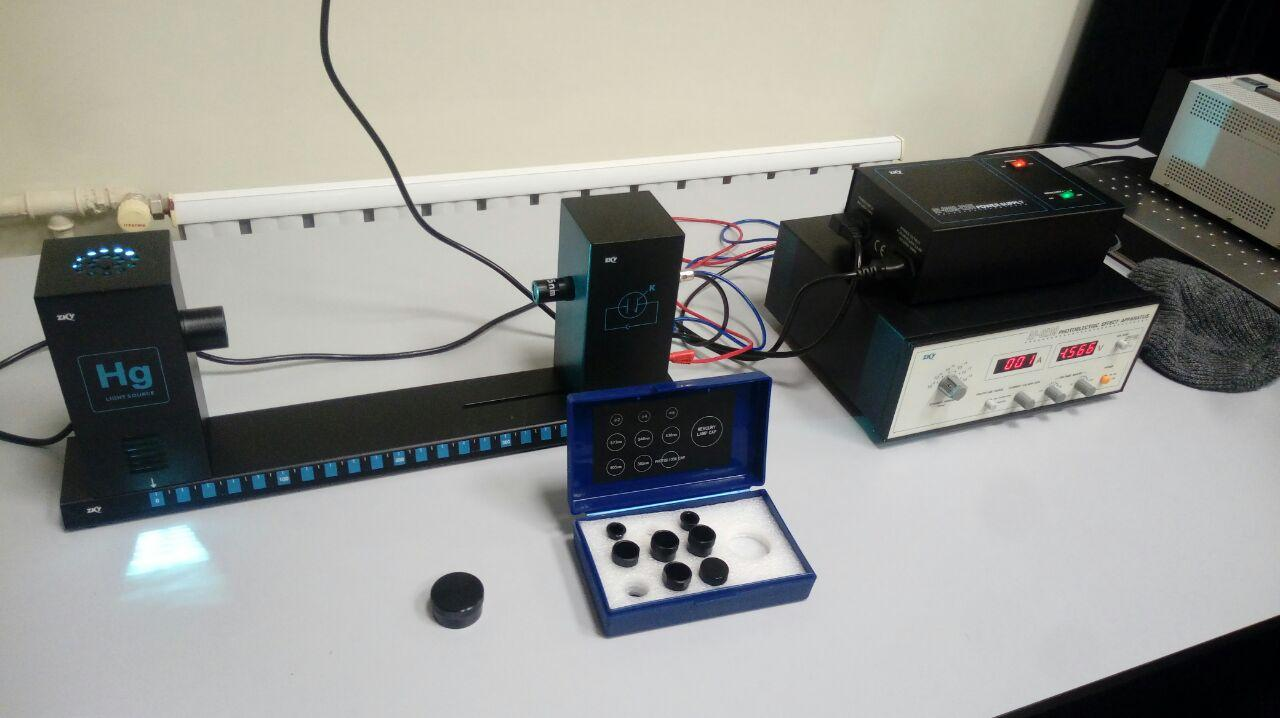
\includegraphics[width=.8\linewidth]{Photoelectric.jpg}
    \caption{The experimental setup}
\end{figure}


From the left, light source, photodiode, filters \& apertures, power supply, and photoelectric effect apparatus. The experimental procedure was the following (change apertures, filters depending on the part):

\begin{enumerate}
    \item Warm-up, let the equipment be warmed up before the experiment
\item Calibration
\item Measurement of Planck's constant and work function
\item Measurement of current-voltage characteristics at different light intensities
\item Measurement of current-voltage characteristics at different light wavelengths
\end{enumerate}

\newpage


\section{Part 2}
\subsection{Theory and Formula Derivations}

\paragraph{}

Write the work function $W_0$ for photoelectric effect, where $KE_{max}$ is the highest amount of energy emitted by electron:
\begin{equation}
    E=hv=KE_{max}+W_0
\end{equation}

If you solve for kinetic energy you would get:

\begin{equation}
    KE_{max}=h\nu-W_0
\end{equation}

In this case $KE_{max}=eV$ and thus:

\begin{equation}
    eV=h\nu-W_0
\end{equation}
\begin{equation}
    V=\frac{h\nu}{e}=\frac{W_0}{e}
\end{equation}

For varying frequency theory predicts $\frac{h}{e}$ to be $\frac{V}{\nu}$, which is the slope of Stopping Potential vs Frequency graph. And work function is product of the shift of the graph and charge of electron.

\paragraph{}


\newpage

\subsection{Analysis}

\paragraph{}

\subsubsection{Part A}

 \begin{figure}[H]
    \centering
    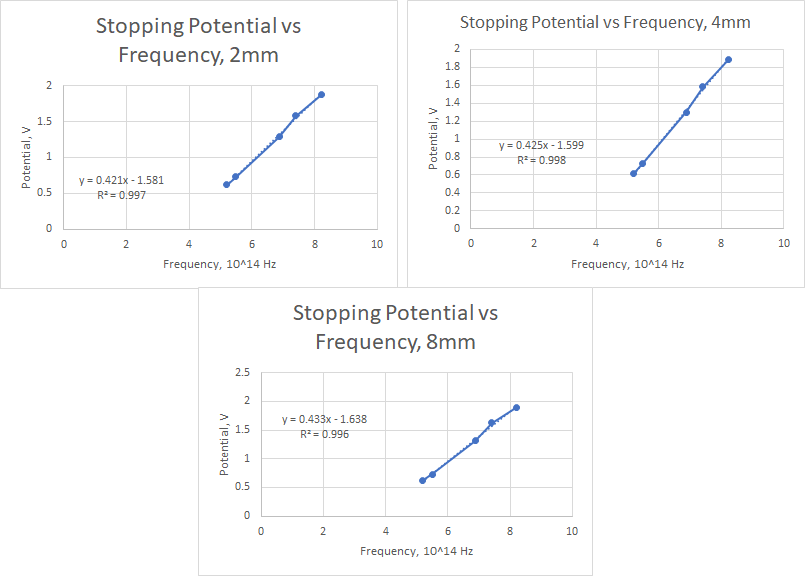
\includegraphics[width=.9\linewidth]{part1lab3.png} 
    \caption{Voltage vs Frequency graphs for 2mm, 4mm, 8mm apertures}
    \label{fig:calib}
    \end{figure}

\begin{table}[H]
       \centering
       \caption{ \textit{Planck's constant and Work Function}}
       \begin{tabular}{| c |c| c |}
       \hline
       Aperture, mm & Planck's constant ($h$), $10^{-34}$J/s& Work Function ($W_0$), eV\\
       \hline
       2 &   $6.811\pm0.35$ &  2.53  \\
       \hline
       4   &  $6.752\pm0.37$   &  2.56  \\
       \hline
       8 &  $6.940\pm0.51$   &  2.63   \\
       \hline
       \end{tabular}
   \end{table}   
   
   
\subsubsection{Part B}


 \begin{figure}[H]
    \centering
    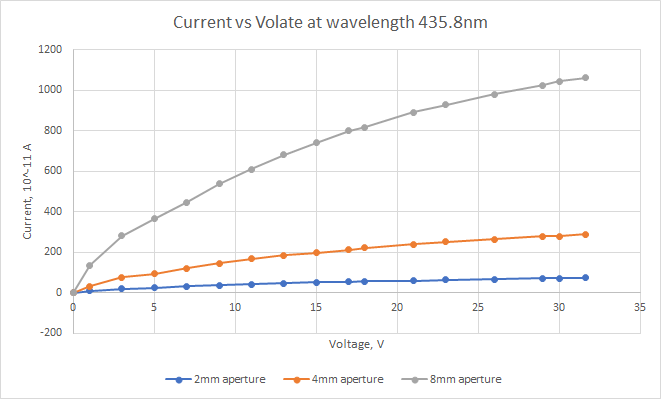
\includegraphics[width=.9\linewidth]{part2lab3.png} 
    \caption{Current vs Voltage at different apertures and constant wavelength}
    \label{fig:calib}
    \end{figure}

\subsubsection{Part C}

 \begin{figure}[H]
    \centering
    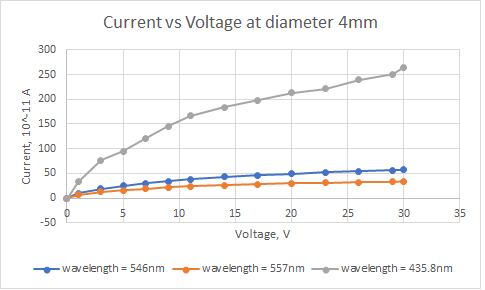
\includegraphics[width=.9\linewidth]{part3lab3.png} 
    \caption{Current vs Voltage at different wavelengths and constant aperture}
    \label{fig:calib}
    \end{figure}

\newpage




\section{Part 3}
\subsection{Experimental data}

\paragraph{}

 \begin{table}
 \centering
  \caption{Part B. Current and Voltage at different apertures and constant wavelength}
 \begin{tabular}{ | c | c | c | c | }
\hline
    & \multicolumn{3}{c}{Current, $10^{-11}$ A}\\ \hline
	Voltage, V &2mm & 4mm & 8mm \\ \hline
	0 & -0.11 & -1.2 & -1.2 \\ \hline
	1 & 10 & 33 & 136 \\ \hline
	3 & 21 & 77 & 282 \\ \hline
	5 & 25 & 95 & 365 \\ \hline
	7 & 32 & 121 & 447 \\ \hline
	9 & 38 & 145 & 539 \\ \hline
	11 & 43 & 167 & 610 \\ \hline
	13 & 47 & 184 & 680 \\ \hline
	15 & 51 & 198 & 740 \\ \hline
	17 & 54 & 213 & 800 \\ \hline
	18 & 56 & 221 & 817 \\ \hline
	21 & 60 & 239 & 890 \\ \hline
	23 & 64 & 251 & 928 \\ \hline
	26 & 67 & 265 & 980 \\ \hline
	29 & 71 & 278 & 1025 \\ \hline
	30 & 72 & 280 & 1045 \\ \hline
	31.6 & 73 & 288 & 1061 \\ \hline
\end{tabular}
\end{table}

 \begin{table}
 \centering
   
 \begin{tabular}{ | c | c | c | c | }
  \caption{Part C. Current and Voltage at different wavelengths and constant apertures}
\hline
    & \multicolumn{3}{c}{Current, $10^{-11}$ A}\\ \hline
	Voltage, V & 546nm & 577nm & 435.8nm \\ \hline
	0 & -0.05 & -0.3 & -1.2 \\ \hline
	1 & 10 & 7 & 33 \\ \hline
	3 & 19 & 13 & 77 \\ \hline
	5 & 25 & 16 & 95 \\ \hline
	7 & 30 & 19 & 121 \\ \hline
	9 & 34 & 22 & 145 \\ \hline
	11 & 38 & 24 & 167 \\ \hline
	14 & 43 & 26 & 184 \\ \hline
	17 & 46 & 28 & 198 \\ \hline
	20 & 49 & 30 & 213 \\ \hline
	23 & 52 & 31 & 221 \\ \hline
	26 & 54 & 32 & 239 \\ \hline
	29 & 56 & 33 & 251 \\ \hline
	30 & 57 & 34 & 265 \\ \hline
\end{tabular}
\end{table}





\newpage
\subsection{Discussion}
\paragraph{Part A} Calculated value for Planck's constant is within reasonable error range and confirms the theoretical values with relative error of $3.14\%$. Work function values range from 2.53 to 2.63, thus Sr, Wb and Ba all work for the obtained range. However, knowing that for Barium the work function values also range from 2.52 to 2.7 we determine, the most probable cathode metal studied in photoelectric effect to be Barium.
\paragraph{Part B} According to Einstein, each photon, hitting the electron, causes it to eject. Thus, according to the theory, graph shows that number of emitted electrons depends on the number of photons and, therefore, the intensity of light.

\paragraph{Part C}  Does the photoelectric effect depend on the frequency of light?

In the graph we observe, that lower wavelengths correspond to higher current, due to the fact that low-wavelength photons have high frequencies. As shown in part B, the number of electrons depends on light intensity and is frequency independent. The Kinetic energy of the electrons, on the other hand, depends on the frequency and is independent of light intensity.




\newpage
\subsection{Conclusion}
\paragraph{}




\newpage






% This is bibliography, DO NOT CHANGE THIS FIELD

% GO to main.bib to edit References

\addcontentsline{toc}{section}{References}
\printbibliography






 
 




\end{document}



